% Created by tikzDevice version 0.12.3.1 on 2021-12-13 20:10:38
% !TEX encoding = UTF-8 Unicode
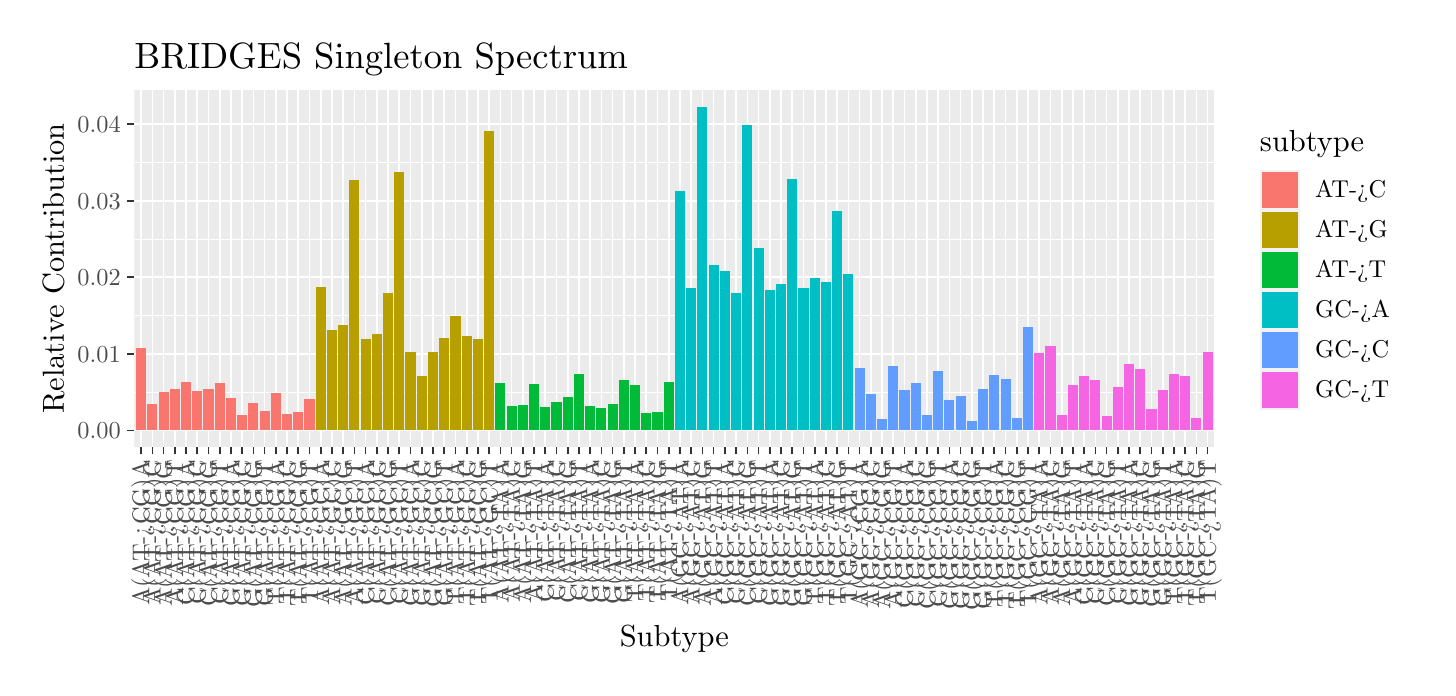
\begin{tikzpicture}[x=1pt,y=1pt]
\definecolor{fillColor}{RGB}{255,255,255}
\path[use as bounding box,fill=fillColor,fill opacity=0.00] (0,0) rectangle (505.89,231.26);
\begin{scope}
\path[clip] (  0.00,  0.00) rectangle (505.89,231.26);
\definecolor{drawColor}{RGB}{255,255,255}
\definecolor{fillColor}{RGB}{255,255,255}

\path[draw=drawColor,line width= 0.6pt,line join=round,line cap=round,fill=fillColor] (  0.00,  0.00) rectangle (505.89,231.26);
\end{scope}
\begin{scope}
\path[clip] ( 38.56, 79.86) rectangle (428.80,208.61);
\definecolor{fillColor}{gray}{0.92}

\path[fill=fillColor] ( 38.56, 79.86) rectangle (428.80,208.61);
\definecolor{drawColor}{RGB}{255,255,255}

\path[draw=drawColor,line width= 0.3pt,line join=round] ( 38.56, 99.55) --
	(428.80, 99.55);

\path[draw=drawColor,line width= 0.3pt,line join=round] ( 38.56,127.22) --
	(428.80,127.22);

\path[draw=drawColor,line width= 0.3pt,line join=round] ( 38.56,154.90) --
	(428.80,154.90);

\path[draw=drawColor,line width= 0.3pt,line join=round] ( 38.56,182.57) --
	(428.80,182.57);

\path[draw=drawColor,line width= 0.6pt,line join=round] ( 38.56, 85.71) --
	(428.80, 85.71);

\path[draw=drawColor,line width= 0.6pt,line join=round] ( 38.56,113.38) --
	(428.80,113.38);

\path[draw=drawColor,line width= 0.6pt,line join=round] ( 38.56,141.06) --
	(428.80,141.06);

\path[draw=drawColor,line width= 0.6pt,line join=round] ( 38.56,168.73) --
	(428.80,168.73);

\path[draw=drawColor,line width= 0.6pt,line join=round] ( 38.56,196.41) --
	(428.80,196.41);

\path[draw=drawColor,line width= 0.6pt,line join=round] ( 40.99, 79.86) --
	( 40.99,208.61);

\path[draw=drawColor,line width= 0.6pt,line join=round] ( 45.05, 79.86) --
	( 45.05,208.61);

\path[draw=drawColor,line width= 0.6pt,line join=round] ( 49.10, 79.86) --
	( 49.10,208.61);

\path[draw=drawColor,line width= 0.6pt,line join=round] ( 53.16, 79.86) --
	( 53.16,208.61);

\path[draw=drawColor,line width= 0.6pt,line join=round] ( 57.22, 79.86) --
	( 57.22,208.61);

\path[draw=drawColor,line width= 0.6pt,line join=round] ( 61.27, 79.86) --
	( 61.27,208.61);

\path[draw=drawColor,line width= 0.6pt,line join=round] ( 65.33, 79.86) --
	( 65.33,208.61);

\path[draw=drawColor,line width= 0.6pt,line join=round] ( 69.39, 79.86) --
	( 69.39,208.61);

\path[draw=drawColor,line width= 0.6pt,line join=round] ( 73.44, 79.86) --
	( 73.44,208.61);

\path[draw=drawColor,line width= 0.6pt,line join=round] ( 77.50, 79.86) --
	( 77.50,208.61);

\path[draw=drawColor,line width= 0.6pt,line join=round] ( 81.56, 79.86) --
	( 81.56,208.61);

\path[draw=drawColor,line width= 0.6pt,line join=round] ( 85.61, 79.86) --
	( 85.61,208.61);

\path[draw=drawColor,line width= 0.6pt,line join=round] ( 89.67, 79.86) --
	( 89.67,208.61);

\path[draw=drawColor,line width= 0.6pt,line join=round] ( 93.73, 79.86) --
	( 93.73,208.61);

\path[draw=drawColor,line width= 0.6pt,line join=round] ( 97.78, 79.86) --
	( 97.78,208.61);

\path[draw=drawColor,line width= 0.6pt,line join=round] (101.84, 79.86) --
	(101.84,208.61);

\path[draw=drawColor,line width= 0.6pt,line join=round] (105.90, 79.86) --
	(105.90,208.61);

\path[draw=drawColor,line width= 0.6pt,line join=round] (109.95, 79.86) --
	(109.95,208.61);

\path[draw=drawColor,line width= 0.6pt,line join=round] (114.01, 79.86) --
	(114.01,208.61);

\path[draw=drawColor,line width= 0.6pt,line join=round] (118.07, 79.86) --
	(118.07,208.61);

\path[draw=drawColor,line width= 0.6pt,line join=round] (122.12, 79.86) --
	(122.12,208.61);

\path[draw=drawColor,line width= 0.6pt,line join=round] (126.18, 79.86) --
	(126.18,208.61);

\path[draw=drawColor,line width= 0.6pt,line join=round] (130.24, 79.86) --
	(130.24,208.61);

\path[draw=drawColor,line width= 0.6pt,line join=round] (134.29, 79.86) --
	(134.29,208.61);

\path[draw=drawColor,line width= 0.6pt,line join=round] (138.35, 79.86) --
	(138.35,208.61);

\path[draw=drawColor,line width= 0.6pt,line join=round] (142.41, 79.86) --
	(142.41,208.61);

\path[draw=drawColor,line width= 0.6pt,line join=round] (146.46, 79.86) --
	(146.46,208.61);

\path[draw=drawColor,line width= 0.6pt,line join=round] (150.52, 79.86) --
	(150.52,208.61);

\path[draw=drawColor,line width= 0.6pt,line join=round] (154.58, 79.86) --
	(154.58,208.61);

\path[draw=drawColor,line width= 0.6pt,line join=round] (158.63, 79.86) --
	(158.63,208.61);

\path[draw=drawColor,line width= 0.6pt,line join=round] (162.69, 79.86) --
	(162.69,208.61);

\path[draw=drawColor,line width= 0.6pt,line join=round] (166.74, 79.86) --
	(166.74,208.61);

\path[draw=drawColor,line width= 0.6pt,line join=round] (170.80, 79.86) --
	(170.80,208.61);

\path[draw=drawColor,line width= 0.6pt,line join=round] (174.86, 79.86) --
	(174.86,208.61);

\path[draw=drawColor,line width= 0.6pt,line join=round] (178.91, 79.86) --
	(178.91,208.61);

\path[draw=drawColor,line width= 0.6pt,line join=round] (182.97, 79.86) --
	(182.97,208.61);

\path[draw=drawColor,line width= 0.6pt,line join=round] (187.03, 79.86) --
	(187.03,208.61);

\path[draw=drawColor,line width= 0.6pt,line join=round] (191.08, 79.86) --
	(191.08,208.61);

\path[draw=drawColor,line width= 0.6pt,line join=round] (195.14, 79.86) --
	(195.14,208.61);

\path[draw=drawColor,line width= 0.6pt,line join=round] (199.20, 79.86) --
	(199.20,208.61);

\path[draw=drawColor,line width= 0.6pt,line join=round] (203.25, 79.86) --
	(203.25,208.61);

\path[draw=drawColor,line width= 0.6pt,line join=round] (207.31, 79.86) --
	(207.31,208.61);

\path[draw=drawColor,line width= 0.6pt,line join=round] (211.37, 79.86) --
	(211.37,208.61);

\path[draw=drawColor,line width= 0.6pt,line join=round] (215.42, 79.86) --
	(215.42,208.61);

\path[draw=drawColor,line width= 0.6pt,line join=round] (219.48, 79.86) --
	(219.48,208.61);

\path[draw=drawColor,line width= 0.6pt,line join=round] (223.54, 79.86) --
	(223.54,208.61);

\path[draw=drawColor,line width= 0.6pt,line join=round] (227.59, 79.86) --
	(227.59,208.61);

\path[draw=drawColor,line width= 0.6pt,line join=round] (231.65, 79.86) --
	(231.65,208.61);

\path[draw=drawColor,line width= 0.6pt,line join=round] (235.71, 79.86) --
	(235.71,208.61);

\path[draw=drawColor,line width= 0.6pt,line join=round] (239.76, 79.86) --
	(239.76,208.61);

\path[draw=drawColor,line width= 0.6pt,line join=round] (243.82, 79.86) --
	(243.82,208.61);

\path[draw=drawColor,line width= 0.6pt,line join=round] (247.88, 79.86) --
	(247.88,208.61);

\path[draw=drawColor,line width= 0.6pt,line join=round] (251.93, 79.86) --
	(251.93,208.61);

\path[draw=drawColor,line width= 0.6pt,line join=round] (255.99, 79.86) --
	(255.99,208.61);

\path[draw=drawColor,line width= 0.6pt,line join=round] (260.05, 79.86) --
	(260.05,208.61);

\path[draw=drawColor,line width= 0.6pt,line join=round] (264.10, 79.86) --
	(264.10,208.61);

\path[draw=drawColor,line width= 0.6pt,line join=round] (268.16, 79.86) --
	(268.16,208.61);

\path[draw=drawColor,line width= 0.6pt,line join=round] (272.22, 79.86) --
	(272.22,208.61);

\path[draw=drawColor,line width= 0.6pt,line join=round] (276.27, 79.86) --
	(276.27,208.61);

\path[draw=drawColor,line width= 0.6pt,line join=round] (280.33, 79.86) --
	(280.33,208.61);

\path[draw=drawColor,line width= 0.6pt,line join=round] (284.39, 79.86) --
	(284.39,208.61);

\path[draw=drawColor,line width= 0.6pt,line join=round] (288.44, 79.86) --
	(288.44,208.61);

\path[draw=drawColor,line width= 0.6pt,line join=round] (292.50, 79.86) --
	(292.50,208.61);

\path[draw=drawColor,line width= 0.6pt,line join=round] (296.56, 79.86) --
	(296.56,208.61);

\path[draw=drawColor,line width= 0.6pt,line join=round] (300.61, 79.86) --
	(300.61,208.61);

\path[draw=drawColor,line width= 0.6pt,line join=round] (304.67, 79.86) --
	(304.67,208.61);

\path[draw=drawColor,line width= 0.6pt,line join=round] (308.73, 79.86) --
	(308.73,208.61);

\path[draw=drawColor,line width= 0.6pt,line join=round] (312.78, 79.86) --
	(312.78,208.61);

\path[draw=drawColor,line width= 0.6pt,line join=round] (316.84, 79.86) --
	(316.84,208.61);

\path[draw=drawColor,line width= 0.6pt,line join=round] (320.90, 79.86) --
	(320.90,208.61);

\path[draw=drawColor,line width= 0.6pt,line join=round] (324.95, 79.86) --
	(324.95,208.61);

\path[draw=drawColor,line width= 0.6pt,line join=round] (329.01, 79.86) --
	(329.01,208.61);

\path[draw=drawColor,line width= 0.6pt,line join=round] (333.07, 79.86) --
	(333.07,208.61);

\path[draw=drawColor,line width= 0.6pt,line join=round] (337.12, 79.86) --
	(337.12,208.61);

\path[draw=drawColor,line width= 0.6pt,line join=round] (341.18, 79.86) --
	(341.18,208.61);

\path[draw=drawColor,line width= 0.6pt,line join=round] (345.24, 79.86) --
	(345.24,208.61);

\path[draw=drawColor,line width= 0.6pt,line join=round] (349.29, 79.86) --
	(349.29,208.61);

\path[draw=drawColor,line width= 0.6pt,line join=round] (353.35, 79.86) --
	(353.35,208.61);

\path[draw=drawColor,line width= 0.6pt,line join=round] (357.41, 79.86) --
	(357.41,208.61);

\path[draw=drawColor,line width= 0.6pt,line join=round] (361.46, 79.86) --
	(361.46,208.61);

\path[draw=drawColor,line width= 0.6pt,line join=round] (365.52, 79.86) --
	(365.52,208.61);

\path[draw=drawColor,line width= 0.6pt,line join=round] (369.58, 79.86) --
	(369.58,208.61);

\path[draw=drawColor,line width= 0.6pt,line join=round] (373.63, 79.86) --
	(373.63,208.61);

\path[draw=drawColor,line width= 0.6pt,line join=round] (377.69, 79.86) --
	(377.69,208.61);

\path[draw=drawColor,line width= 0.6pt,line join=round] (381.75, 79.86) --
	(381.75,208.61);

\path[draw=drawColor,line width= 0.6pt,line join=round] (385.80, 79.86) --
	(385.80,208.61);

\path[draw=drawColor,line width= 0.6pt,line join=round] (389.86, 79.86) --
	(389.86,208.61);

\path[draw=drawColor,line width= 0.6pt,line join=round] (393.92, 79.86) --
	(393.92,208.61);

\path[draw=drawColor,line width= 0.6pt,line join=round] (397.97, 79.86) --
	(397.97,208.61);

\path[draw=drawColor,line width= 0.6pt,line join=round] (402.03, 79.86) --
	(402.03,208.61);

\path[draw=drawColor,line width= 0.6pt,line join=round] (406.09, 79.86) --
	(406.09,208.61);

\path[draw=drawColor,line width= 0.6pt,line join=round] (410.14, 79.86) --
	(410.14,208.61);

\path[draw=drawColor,line width= 0.6pt,line join=round] (414.20, 79.86) --
	(414.20,208.61);

\path[draw=drawColor,line width= 0.6pt,line join=round] (418.26, 79.86) --
	(418.26,208.61);

\path[draw=drawColor,line width= 0.6pt,line join=round] (422.31, 79.86) --
	(422.31,208.61);

\path[draw=drawColor,line width= 0.6pt,line join=round] (426.37, 79.86) --
	(426.37,208.61);
\definecolor{fillColor}{RGB}{248,118,109}

\path[fill=fillColor] ( 39.16, 85.71) rectangle ( 42.81,115.58);

\path[fill=fillColor] ( 43.22, 85.71) rectangle ( 46.87, 95.19);

\path[fill=fillColor] ( 47.28, 85.71) rectangle ( 50.93, 99.57);

\path[fill=fillColor] ( 51.33, 85.71) rectangle ( 54.98,100.75);

\path[fill=fillColor] ( 55.39, 85.71) rectangle ( 59.04,103.08);

\path[fill=fillColor] ( 59.45, 85.71) rectangle ( 63.10, 99.88);

\path[fill=fillColor] ( 63.50, 85.71) rectangle ( 67.15,100.85);

\path[fill=fillColor] ( 67.56, 85.71) rectangle ( 71.21,102.90);

\path[fill=fillColor] ( 71.62, 85.71) rectangle ( 75.27, 97.45);

\path[fill=fillColor] ( 75.67, 85.71) rectangle ( 79.32, 91.16);

\path[fill=fillColor] ( 79.73, 85.71) rectangle ( 83.38, 95.50);

\path[fill=fillColor] ( 83.79, 85.71) rectangle ( 87.44, 92.90);

\path[fill=fillColor] ( 87.84, 85.71) rectangle ( 91.49, 99.17);

\path[fill=fillColor] ( 91.90, 85.71) rectangle ( 95.55, 91.57);

\path[fill=fillColor] ( 95.96, 85.71) rectangle ( 99.61, 92.29);

\path[fill=fillColor] (100.01, 85.71) rectangle (103.66, 97.16);
\definecolor{fillColor}{RGB}{183,159,0}

\path[fill=fillColor] (104.07, 85.71) rectangle (107.72,137.44);

\path[fill=fillColor] (108.13, 85.71) rectangle (111.78,122.14);

\path[fill=fillColor] (112.18, 85.71) rectangle (115.83,123.92);

\path[fill=fillColor] (116.24, 85.71) rectangle (119.89,176.08);

\path[fill=fillColor] (120.30, 85.71) rectangle (123.95,118.68);

\path[fill=fillColor] (124.35, 85.71) rectangle (128.00,120.44);

\path[fill=fillColor] (128.41, 85.71) rectangle (132.06,135.49);

\path[fill=fillColor] (132.47, 85.71) rectangle (136.12,179.07);

\path[fill=fillColor] (136.52, 85.71) rectangle (140.17,113.94);

\path[fill=fillColor] (140.58, 85.71) rectangle (144.23,105.29);

\path[fill=fillColor] (144.64, 85.71) rectangle (148.29,114.15);

\path[fill=fillColor] (148.69, 85.71) rectangle (152.34,119.09);

\path[fill=fillColor] (152.75, 85.71) rectangle (156.40,127.04);

\path[fill=fillColor] (156.81, 85.71) rectangle (160.46,119.69);

\path[fill=fillColor] (160.86, 85.71) rectangle (164.51,118.82);

\path[fill=fillColor] (164.92, 85.71) rectangle (168.57,193.81);
\definecolor{fillColor}{RGB}{0,186,56}

\path[fill=fillColor] (168.98, 85.71) rectangle (172.63,102.82);

\path[fill=fillColor] (173.03, 85.71) rectangle (176.68, 94.63);

\path[fill=fillColor] (177.09, 85.71) rectangle (180.74, 94.99);

\path[fill=fillColor] (181.15, 85.71) rectangle (184.80,102.49);

\path[fill=fillColor] (185.20, 85.71) rectangle (188.85, 94.15);

\path[fill=fillColor] (189.26, 85.71) rectangle (192.91, 96.02);

\path[fill=fillColor] (193.32, 85.71) rectangle (196.97, 97.67);

\path[fill=fillColor] (197.37, 85.71) rectangle (201.02,105.95);

\path[fill=fillColor] (201.43, 85.71) rectangle (205.08, 94.72);

\path[fill=fillColor] (205.49, 85.71) rectangle (209.14, 93.87);

\path[fill=fillColor] (209.54, 85.71) rectangle (213.19, 95.31);

\path[fill=fillColor] (213.60, 85.71) rectangle (217.25,103.89);

\path[fill=fillColor] (217.66, 85.71) rectangle (221.31,102.20);

\path[fill=fillColor] (221.71, 85.71) rectangle (225.36, 92.18);

\path[fill=fillColor] (225.77, 85.71) rectangle (229.42, 92.44);

\path[fill=fillColor] (229.83, 85.71) rectangle (233.48,103.21);
\definecolor{fillColor}{RGB}{0,191,196}

\path[fill=fillColor] (233.88, 85.71) rectangle (237.53,172.25);

\path[fill=fillColor] (237.94, 85.71) rectangle (241.59,137.13);

\path[fill=fillColor] (242.00, 85.71) rectangle (245.65,202.75);

\path[fill=fillColor] (246.05, 85.71) rectangle (249.70,145.55);

\path[fill=fillColor] (250.11, 85.71) rectangle (253.76,143.32);

\path[fill=fillColor] (254.17, 85.71) rectangle (257.82,135.47);

\path[fill=fillColor] (258.22, 85.71) rectangle (261.87,195.93);

\path[fill=fillColor] (262.28, 85.71) rectangle (265.93,151.49);

\path[fill=fillColor] (266.34, 85.71) rectangle (269.99,136.49);

\path[fill=fillColor] (270.39, 85.71) rectangle (274.04,138.75);

\path[fill=fillColor] (274.45, 85.71) rectangle (278.10,176.44);

\path[fill=fillColor] (278.51, 85.71) rectangle (282.16,137.07);

\path[fill=fillColor] (282.56, 85.71) rectangle (286.21,140.73);

\path[fill=fillColor] (286.62, 85.71) rectangle (290.27,139.21);

\path[fill=fillColor] (290.68, 85.71) rectangle (294.33,165.02);

\path[fill=fillColor] (294.73, 85.71) rectangle (298.38,142.37);
\definecolor{fillColor}{RGB}{97,156,255}

\path[fill=fillColor] (298.79, 85.71) rectangle (302.44,108.16);

\path[fill=fillColor] (302.85, 85.71) rectangle (306.50, 98.94);

\path[fill=fillColor] (306.90, 85.71) rectangle (310.55, 90.01);

\path[fill=fillColor] (310.96, 85.71) rectangle (314.61,108.89);

\path[fill=fillColor] (315.02, 85.71) rectangle (318.67,100.17);

\path[fill=fillColor] (319.07, 85.71) rectangle (322.72,103.04);

\path[fill=fillColor] (323.13, 85.71) rectangle (326.78, 91.17);

\path[fill=fillColor] (327.19, 85.71) rectangle (330.84,107.11);

\path[fill=fillColor] (331.24, 85.71) rectangle (334.89, 96.81);

\path[fill=fillColor] (335.30, 85.71) rectangle (338.95, 98.11);

\path[fill=fillColor] (339.36, 85.71) rectangle (343.01, 89.09);

\path[fill=fillColor] (343.41, 85.71) rectangle (347.06,100.52);

\path[fill=fillColor] (347.47, 85.71) rectangle (351.12,105.81);

\path[fill=fillColor] (351.53, 85.71) rectangle (355.18,104.31);

\path[fill=fillColor] (355.58, 85.71) rectangle (359.23, 90.35);

\path[fill=fillColor] (359.64, 85.71) rectangle (363.29,123.06);
\definecolor{fillColor}{RGB}{245,100,227}

\path[fill=fillColor] (363.70, 85.71) rectangle (367.35,113.87);

\path[fill=fillColor] (367.75, 85.71) rectangle (371.40,116.09);

\path[fill=fillColor] (371.81, 85.71) rectangle (375.46, 91.38);

\path[fill=fillColor] (375.86, 85.71) rectangle (379.52,102.15);

\path[fill=fillColor] (379.92, 85.71) rectangle (383.57,105.44);

\path[fill=fillColor] (383.98, 85.71) rectangle (387.63,104.11);

\path[fill=fillColor] (388.03, 85.71) rectangle (391.69, 91.04);

\path[fill=fillColor] (392.09, 85.71) rectangle (395.74,101.54);

\path[fill=fillColor] (396.15, 85.71) rectangle (399.80,109.88);

\path[fill=fillColor] (400.20, 85.71) rectangle (403.86,108.05);

\path[fill=fillColor] (404.26, 85.71) rectangle (407.91, 93.58);

\path[fill=fillColor] (408.32, 85.71) rectangle (411.97,100.33);

\path[fill=fillColor] (412.37, 85.71) rectangle (416.03,106.26);

\path[fill=fillColor] (416.43, 85.71) rectangle (420.08,105.43);

\path[fill=fillColor] (420.49, 85.71) rectangle (424.14, 90.21);

\path[fill=fillColor] (424.54, 85.71) rectangle (428.20,113.99);
\end{scope}
\begin{scope}
\path[clip] (  0.00,  0.00) rectangle (505.89,231.26);
\definecolor{drawColor}{gray}{0.30}

\node[text=drawColor,anchor=base east,inner sep=0pt, outer sep=0pt, scale=  0.88] at ( 33.61, 82.68) {0.00};

\node[text=drawColor,anchor=base east,inner sep=0pt, outer sep=0pt, scale=  0.88] at ( 33.61,110.35) {0.01};

\node[text=drawColor,anchor=base east,inner sep=0pt, outer sep=0pt, scale=  0.88] at ( 33.61,138.03) {0.02};

\node[text=drawColor,anchor=base east,inner sep=0pt, outer sep=0pt, scale=  0.88] at ( 33.61,165.70) {0.03};

\node[text=drawColor,anchor=base east,inner sep=0pt, outer sep=0pt, scale=  0.88] at ( 33.61,193.38) {0.04};
\end{scope}
\begin{scope}
\path[clip] (  0.00,  0.00) rectangle (505.89,231.26);
\definecolor{drawColor}{gray}{0.20}

\path[draw=drawColor,line width= 0.6pt,line join=round] ( 35.81, 85.71) --
	( 38.56, 85.71);

\path[draw=drawColor,line width= 0.6pt,line join=round] ( 35.81,113.38) --
	( 38.56,113.38);

\path[draw=drawColor,line width= 0.6pt,line join=round] ( 35.81,141.06) --
	( 38.56,141.06);

\path[draw=drawColor,line width= 0.6pt,line join=round] ( 35.81,168.73) --
	( 38.56,168.73);

\path[draw=drawColor,line width= 0.6pt,line join=round] ( 35.81,196.41) --
	( 38.56,196.41);
\end{scope}
\begin{scope}
\path[clip] (  0.00,  0.00) rectangle (505.89,231.26);
\definecolor{drawColor}{gray}{0.20}

\path[draw=drawColor,line width= 0.6pt,line join=round] ( 40.99, 77.11) --
	( 40.99, 79.86);

\path[draw=drawColor,line width= 0.6pt,line join=round] ( 45.05, 77.11) --
	( 45.05, 79.86);

\path[draw=drawColor,line width= 0.6pt,line join=round] ( 49.10, 77.11) --
	( 49.10, 79.86);

\path[draw=drawColor,line width= 0.6pt,line join=round] ( 53.16, 77.11) --
	( 53.16, 79.86);

\path[draw=drawColor,line width= 0.6pt,line join=round] ( 57.22, 77.11) --
	( 57.22, 79.86);

\path[draw=drawColor,line width= 0.6pt,line join=round] ( 61.27, 77.11) --
	( 61.27, 79.86);

\path[draw=drawColor,line width= 0.6pt,line join=round] ( 65.33, 77.11) --
	( 65.33, 79.86);

\path[draw=drawColor,line width= 0.6pt,line join=round] ( 69.39, 77.11) --
	( 69.39, 79.86);

\path[draw=drawColor,line width= 0.6pt,line join=round] ( 73.44, 77.11) --
	( 73.44, 79.86);

\path[draw=drawColor,line width= 0.6pt,line join=round] ( 77.50, 77.11) --
	( 77.50, 79.86);

\path[draw=drawColor,line width= 0.6pt,line join=round] ( 81.56, 77.11) --
	( 81.56, 79.86);

\path[draw=drawColor,line width= 0.6pt,line join=round] ( 85.61, 77.11) --
	( 85.61, 79.86);

\path[draw=drawColor,line width= 0.6pt,line join=round] ( 89.67, 77.11) --
	( 89.67, 79.86);

\path[draw=drawColor,line width= 0.6pt,line join=round] ( 93.73, 77.11) --
	( 93.73, 79.86);

\path[draw=drawColor,line width= 0.6pt,line join=round] ( 97.78, 77.11) --
	( 97.78, 79.86);

\path[draw=drawColor,line width= 0.6pt,line join=round] (101.84, 77.11) --
	(101.84, 79.86);

\path[draw=drawColor,line width= 0.6pt,line join=round] (105.90, 77.11) --
	(105.90, 79.86);

\path[draw=drawColor,line width= 0.6pt,line join=round] (109.95, 77.11) --
	(109.95, 79.86);

\path[draw=drawColor,line width= 0.6pt,line join=round] (114.01, 77.11) --
	(114.01, 79.86);

\path[draw=drawColor,line width= 0.6pt,line join=round] (118.07, 77.11) --
	(118.07, 79.86);

\path[draw=drawColor,line width= 0.6pt,line join=round] (122.12, 77.11) --
	(122.12, 79.86);

\path[draw=drawColor,line width= 0.6pt,line join=round] (126.18, 77.11) --
	(126.18, 79.86);

\path[draw=drawColor,line width= 0.6pt,line join=round] (130.24, 77.11) --
	(130.24, 79.86);

\path[draw=drawColor,line width= 0.6pt,line join=round] (134.29, 77.11) --
	(134.29, 79.86);

\path[draw=drawColor,line width= 0.6pt,line join=round] (138.35, 77.11) --
	(138.35, 79.86);

\path[draw=drawColor,line width= 0.6pt,line join=round] (142.41, 77.11) --
	(142.41, 79.86);

\path[draw=drawColor,line width= 0.6pt,line join=round] (146.46, 77.11) --
	(146.46, 79.86);

\path[draw=drawColor,line width= 0.6pt,line join=round] (150.52, 77.11) --
	(150.52, 79.86);

\path[draw=drawColor,line width= 0.6pt,line join=round] (154.58, 77.11) --
	(154.58, 79.86);

\path[draw=drawColor,line width= 0.6pt,line join=round] (158.63, 77.11) --
	(158.63, 79.86);

\path[draw=drawColor,line width= 0.6pt,line join=round] (162.69, 77.11) --
	(162.69, 79.86);

\path[draw=drawColor,line width= 0.6pt,line join=round] (166.74, 77.11) --
	(166.74, 79.86);

\path[draw=drawColor,line width= 0.6pt,line join=round] (170.80, 77.11) --
	(170.80, 79.86);

\path[draw=drawColor,line width= 0.6pt,line join=round] (174.86, 77.11) --
	(174.86, 79.86);

\path[draw=drawColor,line width= 0.6pt,line join=round] (178.91, 77.11) --
	(178.91, 79.86);

\path[draw=drawColor,line width= 0.6pt,line join=round] (182.97, 77.11) --
	(182.97, 79.86);

\path[draw=drawColor,line width= 0.6pt,line join=round] (187.03, 77.11) --
	(187.03, 79.86);

\path[draw=drawColor,line width= 0.6pt,line join=round] (191.08, 77.11) --
	(191.08, 79.86);

\path[draw=drawColor,line width= 0.6pt,line join=round] (195.14, 77.11) --
	(195.14, 79.86);

\path[draw=drawColor,line width= 0.6pt,line join=round] (199.20, 77.11) --
	(199.20, 79.86);

\path[draw=drawColor,line width= 0.6pt,line join=round] (203.25, 77.11) --
	(203.25, 79.86);

\path[draw=drawColor,line width= 0.6pt,line join=round] (207.31, 77.11) --
	(207.31, 79.86);

\path[draw=drawColor,line width= 0.6pt,line join=round] (211.37, 77.11) --
	(211.37, 79.86);

\path[draw=drawColor,line width= 0.6pt,line join=round] (215.42, 77.11) --
	(215.42, 79.86);

\path[draw=drawColor,line width= 0.6pt,line join=round] (219.48, 77.11) --
	(219.48, 79.86);

\path[draw=drawColor,line width= 0.6pt,line join=round] (223.54, 77.11) --
	(223.54, 79.86);

\path[draw=drawColor,line width= 0.6pt,line join=round] (227.59, 77.11) --
	(227.59, 79.86);

\path[draw=drawColor,line width= 0.6pt,line join=round] (231.65, 77.11) --
	(231.65, 79.86);

\path[draw=drawColor,line width= 0.6pt,line join=round] (235.71, 77.11) --
	(235.71, 79.86);

\path[draw=drawColor,line width= 0.6pt,line join=round] (239.76, 77.11) --
	(239.76, 79.86);

\path[draw=drawColor,line width= 0.6pt,line join=round] (243.82, 77.11) --
	(243.82, 79.86);

\path[draw=drawColor,line width= 0.6pt,line join=round] (247.88, 77.11) --
	(247.88, 79.86);

\path[draw=drawColor,line width= 0.6pt,line join=round] (251.93, 77.11) --
	(251.93, 79.86);

\path[draw=drawColor,line width= 0.6pt,line join=round] (255.99, 77.11) --
	(255.99, 79.86);

\path[draw=drawColor,line width= 0.6pt,line join=round] (260.05, 77.11) --
	(260.05, 79.86);

\path[draw=drawColor,line width= 0.6pt,line join=round] (264.10, 77.11) --
	(264.10, 79.86);

\path[draw=drawColor,line width= 0.6pt,line join=round] (268.16, 77.11) --
	(268.16, 79.86);

\path[draw=drawColor,line width= 0.6pt,line join=round] (272.22, 77.11) --
	(272.22, 79.86);

\path[draw=drawColor,line width= 0.6pt,line join=round] (276.27, 77.11) --
	(276.27, 79.86);

\path[draw=drawColor,line width= 0.6pt,line join=round] (280.33, 77.11) --
	(280.33, 79.86);

\path[draw=drawColor,line width= 0.6pt,line join=round] (284.39, 77.11) --
	(284.39, 79.86);

\path[draw=drawColor,line width= 0.6pt,line join=round] (288.44, 77.11) --
	(288.44, 79.86);

\path[draw=drawColor,line width= 0.6pt,line join=round] (292.50, 77.11) --
	(292.50, 79.86);

\path[draw=drawColor,line width= 0.6pt,line join=round] (296.56, 77.11) --
	(296.56, 79.86);

\path[draw=drawColor,line width= 0.6pt,line join=round] (300.61, 77.11) --
	(300.61, 79.86);

\path[draw=drawColor,line width= 0.6pt,line join=round] (304.67, 77.11) --
	(304.67, 79.86);

\path[draw=drawColor,line width= 0.6pt,line join=round] (308.73, 77.11) --
	(308.73, 79.86);

\path[draw=drawColor,line width= 0.6pt,line join=round] (312.78, 77.11) --
	(312.78, 79.86);

\path[draw=drawColor,line width= 0.6pt,line join=round] (316.84, 77.11) --
	(316.84, 79.86);

\path[draw=drawColor,line width= 0.6pt,line join=round] (320.90, 77.11) --
	(320.90, 79.86);

\path[draw=drawColor,line width= 0.6pt,line join=round] (324.95, 77.11) --
	(324.95, 79.86);

\path[draw=drawColor,line width= 0.6pt,line join=round] (329.01, 77.11) --
	(329.01, 79.86);

\path[draw=drawColor,line width= 0.6pt,line join=round] (333.07, 77.11) --
	(333.07, 79.86);

\path[draw=drawColor,line width= 0.6pt,line join=round] (337.12, 77.11) --
	(337.12, 79.86);

\path[draw=drawColor,line width= 0.6pt,line join=round] (341.18, 77.11) --
	(341.18, 79.86);

\path[draw=drawColor,line width= 0.6pt,line join=round] (345.24, 77.11) --
	(345.24, 79.86);

\path[draw=drawColor,line width= 0.6pt,line join=round] (349.29, 77.11) --
	(349.29, 79.86);

\path[draw=drawColor,line width= 0.6pt,line join=round] (353.35, 77.11) --
	(353.35, 79.86);

\path[draw=drawColor,line width= 0.6pt,line join=round] (357.41, 77.11) --
	(357.41, 79.86);

\path[draw=drawColor,line width= 0.6pt,line join=round] (361.46, 77.11) --
	(361.46, 79.86);

\path[draw=drawColor,line width= 0.6pt,line join=round] (365.52, 77.11) --
	(365.52, 79.86);

\path[draw=drawColor,line width= 0.6pt,line join=round] (369.58, 77.11) --
	(369.58, 79.86);

\path[draw=drawColor,line width= 0.6pt,line join=round] (373.63, 77.11) --
	(373.63, 79.86);

\path[draw=drawColor,line width= 0.6pt,line join=round] (377.69, 77.11) --
	(377.69, 79.86);

\path[draw=drawColor,line width= 0.6pt,line join=round] (381.75, 77.11) --
	(381.75, 79.86);

\path[draw=drawColor,line width= 0.6pt,line join=round] (385.80, 77.11) --
	(385.80, 79.86);

\path[draw=drawColor,line width= 0.6pt,line join=round] (389.86, 77.11) --
	(389.86, 79.86);

\path[draw=drawColor,line width= 0.6pt,line join=round] (393.92, 77.11) --
	(393.92, 79.86);

\path[draw=drawColor,line width= 0.6pt,line join=round] (397.97, 77.11) --
	(397.97, 79.86);

\path[draw=drawColor,line width= 0.6pt,line join=round] (402.03, 77.11) --
	(402.03, 79.86);

\path[draw=drawColor,line width= 0.6pt,line join=round] (406.09, 77.11) --
	(406.09, 79.86);

\path[draw=drawColor,line width= 0.6pt,line join=round] (410.14, 77.11) --
	(410.14, 79.86);

\path[draw=drawColor,line width= 0.6pt,line join=round] (414.20, 77.11) --
	(414.20, 79.86);

\path[draw=drawColor,line width= 0.6pt,line join=round] (418.26, 77.11) --
	(418.26, 79.86);

\path[draw=drawColor,line width= 0.6pt,line join=round] (422.31, 77.11) --
	(422.31, 79.86);

\path[draw=drawColor,line width= 0.6pt,line join=round] (426.37, 77.11) --
	(426.37, 79.86);
\end{scope}
\begin{scope}
\path[clip] (  0.00,  0.00) rectangle (505.89,231.26);
\definecolor{drawColor}{gray}{0.30}

\node[text=drawColor,rotate= 90.00,anchor=base east,inner sep=0pt, outer sep=0pt, scale=  0.88] at ( 44.02, 74.91) {A(AT->CG)A};

\node[text=drawColor,rotate= 90.00,anchor=base east,inner sep=0pt, outer sep=0pt, scale=  0.88] at ( 48.08, 74.91) {A(AT->CG)C};

\node[text=drawColor,rotate= 90.00,anchor=base east,inner sep=0pt, outer sep=0pt, scale=  0.88] at ( 52.13, 74.91) {A(AT->CG)G};

\node[text=drawColor,rotate= 90.00,anchor=base east,inner sep=0pt, outer sep=0pt, scale=  0.88] at ( 56.19, 74.91) {A(AT->CG)T};

\node[text=drawColor,rotate= 90.00,anchor=base east,inner sep=0pt, outer sep=0pt, scale=  0.88] at ( 60.25, 74.91) {C(AT->CG)A};

\node[text=drawColor,rotate= 90.00,anchor=base east,inner sep=0pt, outer sep=0pt, scale=  0.88] at ( 64.30, 74.91) {C(AT->CG)C};

\node[text=drawColor,rotate= 90.00,anchor=base east,inner sep=0pt, outer sep=0pt, scale=  0.88] at ( 68.36, 74.91) {C(AT->CG)G};

\node[text=drawColor,rotate= 90.00,anchor=base east,inner sep=0pt, outer sep=0pt, scale=  0.88] at ( 72.42, 74.91) {C(AT->CG)T};

\node[text=drawColor,rotate= 90.00,anchor=base east,inner sep=0pt, outer sep=0pt, scale=  0.88] at ( 76.47, 74.91) {G(AT->CG)A};

\node[text=drawColor,rotate= 90.00,anchor=base east,inner sep=0pt, outer sep=0pt, scale=  0.88] at ( 80.53, 74.91) {G(AT->CG)C};

\node[text=drawColor,rotate= 90.00,anchor=base east,inner sep=0pt, outer sep=0pt, scale=  0.88] at ( 84.59, 74.91) {G(AT->CG)G};

\node[text=drawColor,rotate= 90.00,anchor=base east,inner sep=0pt, outer sep=0pt, scale=  0.88] at ( 88.64, 74.91) {G(AT->CG)T};

\node[text=drawColor,rotate= 90.00,anchor=base east,inner sep=0pt, outer sep=0pt, scale=  0.88] at ( 92.70, 74.91) {T(AT->CG)A};

\node[text=drawColor,rotate= 90.00,anchor=base east,inner sep=0pt, outer sep=0pt, scale=  0.88] at ( 96.76, 74.91) {T(AT->CG)C};

\node[text=drawColor,rotate= 90.00,anchor=base east,inner sep=0pt, outer sep=0pt, scale=  0.88] at (100.81, 74.91) {T(AT->CG)G};

\node[text=drawColor,rotate= 90.00,anchor=base east,inner sep=0pt, outer sep=0pt, scale=  0.88] at (104.87, 74.91) {T(AT->CG)T};

\node[text=drawColor,rotate= 90.00,anchor=base east,inner sep=0pt, outer sep=0pt, scale=  0.88] at (108.93, 74.91) {A(AT->GC)A};

\node[text=drawColor,rotate= 90.00,anchor=base east,inner sep=0pt, outer sep=0pt, scale=  0.88] at (112.98, 74.91) {A(AT->GC)C};

\node[text=drawColor,rotate= 90.00,anchor=base east,inner sep=0pt, outer sep=0pt, scale=  0.88] at (117.04, 74.91) {A(AT->GC)G};

\node[text=drawColor,rotate= 90.00,anchor=base east,inner sep=0pt, outer sep=0pt, scale=  0.88] at (121.10, 74.91) {A(AT->GC)T};

\node[text=drawColor,rotate= 90.00,anchor=base east,inner sep=0pt, outer sep=0pt, scale=  0.88] at (125.15, 74.91) {C(AT->GC)A};

\node[text=drawColor,rotate= 90.00,anchor=base east,inner sep=0pt, outer sep=0pt, scale=  0.88] at (129.21, 74.91) {C(AT->GC)C};

\node[text=drawColor,rotate= 90.00,anchor=base east,inner sep=0pt, outer sep=0pt, scale=  0.88] at (133.27, 74.91) {C(AT->GC)G};

\node[text=drawColor,rotate= 90.00,anchor=base east,inner sep=0pt, outer sep=0pt, scale=  0.88] at (137.32, 74.91) {C(AT->GC)T};

\node[text=drawColor,rotate= 90.00,anchor=base east,inner sep=0pt, outer sep=0pt, scale=  0.88] at (141.38, 74.91) {G(AT->GC)A};

\node[text=drawColor,rotate= 90.00,anchor=base east,inner sep=0pt, outer sep=0pt, scale=  0.88] at (145.44, 74.91) {G(AT->GC)C};

\node[text=drawColor,rotate= 90.00,anchor=base east,inner sep=0pt, outer sep=0pt, scale=  0.88] at (149.49, 74.91) {G(AT->GC)G};

\node[text=drawColor,rotate= 90.00,anchor=base east,inner sep=0pt, outer sep=0pt, scale=  0.88] at (153.55, 74.91) {G(AT->GC)T};

\node[text=drawColor,rotate= 90.00,anchor=base east,inner sep=0pt, outer sep=0pt, scale=  0.88] at (157.61, 74.91) {T(AT->GC)A};

\node[text=drawColor,rotate= 90.00,anchor=base east,inner sep=0pt, outer sep=0pt, scale=  0.88] at (161.66, 74.91) {T(AT->GC)C};

\node[text=drawColor,rotate= 90.00,anchor=base east,inner sep=0pt, outer sep=0pt, scale=  0.88] at (165.72, 74.91) {T(AT->GC)G};

\node[text=drawColor,rotate= 90.00,anchor=base east,inner sep=0pt, outer sep=0pt, scale=  0.88] at (169.78, 74.91) {T(AT->GC)T};

\node[text=drawColor,rotate= 90.00,anchor=base east,inner sep=0pt, outer sep=0pt, scale=  0.88] at (173.83, 74.91) {A(AT->TA)A};

\node[text=drawColor,rotate= 90.00,anchor=base east,inner sep=0pt, outer sep=0pt, scale=  0.88] at (177.89, 74.91) {A(AT->TA)C};

\node[text=drawColor,rotate= 90.00,anchor=base east,inner sep=0pt, outer sep=0pt, scale=  0.88] at (181.95, 74.91) {A(AT->TA)G};

\node[text=drawColor,rotate= 90.00,anchor=base east,inner sep=0pt, outer sep=0pt, scale=  0.88] at (186.00, 74.91) {A(AT->TA)T};

\node[text=drawColor,rotate= 90.00,anchor=base east,inner sep=0pt, outer sep=0pt, scale=  0.88] at (190.06, 74.91) {C(AT->TA)A};

\node[text=drawColor,rotate= 90.00,anchor=base east,inner sep=0pt, outer sep=0pt, scale=  0.88] at (194.12, 74.91) {C(AT->TA)C};

\node[text=drawColor,rotate= 90.00,anchor=base east,inner sep=0pt, outer sep=0pt, scale=  0.88] at (198.17, 74.91) {C(AT->TA)G};

\node[text=drawColor,rotate= 90.00,anchor=base east,inner sep=0pt, outer sep=0pt, scale=  0.88] at (202.23, 74.91) {C(AT->TA)T};

\node[text=drawColor,rotate= 90.00,anchor=base east,inner sep=0pt, outer sep=0pt, scale=  0.88] at (206.29, 74.91) {G(AT->TA)A};

\node[text=drawColor,rotate= 90.00,anchor=base east,inner sep=0pt, outer sep=0pt, scale=  0.88] at (210.34, 74.91) {G(AT->TA)C};

\node[text=drawColor,rotate= 90.00,anchor=base east,inner sep=0pt, outer sep=0pt, scale=  0.88] at (214.40, 74.91) {G(AT->TA)G};

\node[text=drawColor,rotate= 90.00,anchor=base east,inner sep=0pt, outer sep=0pt, scale=  0.88] at (218.46, 74.91) {G(AT->TA)T};

\node[text=drawColor,rotate= 90.00,anchor=base east,inner sep=0pt, outer sep=0pt, scale=  0.88] at (222.51, 74.91) {T(AT->TA)A};

\node[text=drawColor,rotate= 90.00,anchor=base east,inner sep=0pt, outer sep=0pt, scale=  0.88] at (226.57, 74.91) {T(AT->TA)C};

\node[text=drawColor,rotate= 90.00,anchor=base east,inner sep=0pt, outer sep=0pt, scale=  0.88] at (230.63, 74.91) {T(AT->TA)G};

\node[text=drawColor,rotate= 90.00,anchor=base east,inner sep=0pt, outer sep=0pt, scale=  0.88] at (234.68, 74.91) {T(AT->TA)T};

\node[text=drawColor,rotate= 90.00,anchor=base east,inner sep=0pt, outer sep=0pt, scale=  0.88] at (238.74, 74.91) {A(GC->AT)A};

\node[text=drawColor,rotate= 90.00,anchor=base east,inner sep=0pt, outer sep=0pt, scale=  0.88] at (242.79, 74.91) {A(GC->AT)C};

\node[text=drawColor,rotate= 90.00,anchor=base east,inner sep=0pt, outer sep=0pt, scale=  0.88] at (246.85, 74.91) {A(GC->AT)G};

\node[text=drawColor,rotate= 90.00,anchor=base east,inner sep=0pt, outer sep=0pt, scale=  0.88] at (250.91, 74.91) {A(GC->AT)T};

\node[text=drawColor,rotate= 90.00,anchor=base east,inner sep=0pt, outer sep=0pt, scale=  0.88] at (254.96, 74.91) {C(GC->AT)A};

\node[text=drawColor,rotate= 90.00,anchor=base east,inner sep=0pt, outer sep=0pt, scale=  0.88] at (259.02, 74.91) {C(GC->AT)C};

\node[text=drawColor,rotate= 90.00,anchor=base east,inner sep=0pt, outer sep=0pt, scale=  0.88] at (263.08, 74.91) {C(GC->AT)G};

\node[text=drawColor,rotate= 90.00,anchor=base east,inner sep=0pt, outer sep=0pt, scale=  0.88] at (267.13, 74.91) {C(GC->AT)T};

\node[text=drawColor,rotate= 90.00,anchor=base east,inner sep=0pt, outer sep=0pt, scale=  0.88] at (271.19, 74.91) {G(GC->AT)A};

\node[text=drawColor,rotate= 90.00,anchor=base east,inner sep=0pt, outer sep=0pt, scale=  0.88] at (275.25, 74.91) {G(GC->AT)C};

\node[text=drawColor,rotate= 90.00,anchor=base east,inner sep=0pt, outer sep=0pt, scale=  0.88] at (279.30, 74.91) {G(GC->AT)G};

\node[text=drawColor,rotate= 90.00,anchor=base east,inner sep=0pt, outer sep=0pt, scale=  0.88] at (283.36, 74.91) {G(GC->AT)T};

\node[text=drawColor,rotate= 90.00,anchor=base east,inner sep=0pt, outer sep=0pt, scale=  0.88] at (287.42, 74.91) {T(GC->AT)A};

\node[text=drawColor,rotate= 90.00,anchor=base east,inner sep=0pt, outer sep=0pt, scale=  0.88] at (291.47, 74.91) {T(GC->AT)C};

\node[text=drawColor,rotate= 90.00,anchor=base east,inner sep=0pt, outer sep=0pt, scale=  0.88] at (295.53, 74.91) {T(GC->AT)G};

\node[text=drawColor,rotate= 90.00,anchor=base east,inner sep=0pt, outer sep=0pt, scale=  0.88] at (299.59, 74.91) {T(GC->AT)T};

\node[text=drawColor,rotate= 90.00,anchor=base east,inner sep=0pt, outer sep=0pt, scale=  0.88] at (303.64, 74.91) {A(GC->CG)A};

\node[text=drawColor,rotate= 90.00,anchor=base east,inner sep=0pt, outer sep=0pt, scale=  0.88] at (307.70, 74.91) {A(GC->CG)C};

\node[text=drawColor,rotate= 90.00,anchor=base east,inner sep=0pt, outer sep=0pt, scale=  0.88] at (311.76, 74.91) {A(GC->CG)G};

\node[text=drawColor,rotate= 90.00,anchor=base east,inner sep=0pt, outer sep=0pt, scale=  0.88] at (315.81, 74.91) {A(GC->CG)T};

\node[text=drawColor,rotate= 90.00,anchor=base east,inner sep=0pt, outer sep=0pt, scale=  0.88] at (319.87, 74.91) {C(GC->CG)A};

\node[text=drawColor,rotate= 90.00,anchor=base east,inner sep=0pt, outer sep=0pt, scale=  0.88] at (323.93, 74.91) {C(GC->CG)C};

\node[text=drawColor,rotate= 90.00,anchor=base east,inner sep=0pt, outer sep=0pt, scale=  0.88] at (327.98, 74.91) {C(GC->CG)G};

\node[text=drawColor,rotate= 90.00,anchor=base east,inner sep=0pt, outer sep=0pt, scale=  0.88] at (332.04, 74.91) {C(GC->CG)T};

\node[text=drawColor,rotate= 90.00,anchor=base east,inner sep=0pt, outer sep=0pt, scale=  0.88] at (336.10, 74.91) {G(GC->CG)A};

\node[text=drawColor,rotate= 90.00,anchor=base east,inner sep=0pt, outer sep=0pt, scale=  0.88] at (340.15, 74.91) {G(GC->CG)C};

\node[text=drawColor,rotate= 90.00,anchor=base east,inner sep=0pt, outer sep=0pt, scale=  0.88] at (344.21, 74.91) {G(GC->CG)G};

\node[text=drawColor,rotate= 90.00,anchor=base east,inner sep=0pt, outer sep=0pt, scale=  0.88] at (348.27, 74.91) {G(GC->CG)T};

\node[text=drawColor,rotate= 90.00,anchor=base east,inner sep=0pt, outer sep=0pt, scale=  0.88] at (352.32, 74.91) {T(GC->CG)A};

\node[text=drawColor,rotate= 90.00,anchor=base east,inner sep=0pt, outer sep=0pt, scale=  0.88] at (356.38, 74.91) {T(GC->CG)C};

\node[text=drawColor,rotate= 90.00,anchor=base east,inner sep=0pt, outer sep=0pt, scale=  0.88] at (360.44, 74.91) {T(GC->CG)G};

\node[text=drawColor,rotate= 90.00,anchor=base east,inner sep=0pt, outer sep=0pt, scale=  0.88] at (364.49, 74.91) {T(GC->CG)T};

\node[text=drawColor,rotate= 90.00,anchor=base east,inner sep=0pt, outer sep=0pt, scale=  0.88] at (368.55, 74.91) {A(GC->TA)A};

\node[text=drawColor,rotate= 90.00,anchor=base east,inner sep=0pt, outer sep=0pt, scale=  0.88] at (372.61, 74.91) {A(GC->TA)C};

\node[text=drawColor,rotate= 90.00,anchor=base east,inner sep=0pt, outer sep=0pt, scale=  0.88] at (376.66, 74.91) {A(GC->TA)G};

\node[text=drawColor,rotate= 90.00,anchor=base east,inner sep=0pt, outer sep=0pt, scale=  0.88] at (380.72, 74.91) {A(GC->TA)T};

\node[text=drawColor,rotate= 90.00,anchor=base east,inner sep=0pt, outer sep=0pt, scale=  0.88] at (384.78, 74.91) {C(GC->TA)A};

\node[text=drawColor,rotate= 90.00,anchor=base east,inner sep=0pt, outer sep=0pt, scale=  0.88] at (388.83, 74.91) {C(GC->TA)C};

\node[text=drawColor,rotate= 90.00,anchor=base east,inner sep=0pt, outer sep=0pt, scale=  0.88] at (392.89, 74.91) {C(GC->TA)G};

\node[text=drawColor,rotate= 90.00,anchor=base east,inner sep=0pt, outer sep=0pt, scale=  0.88] at (396.95, 74.91) {C(GC->TA)T};

\node[text=drawColor,rotate= 90.00,anchor=base east,inner sep=0pt, outer sep=0pt, scale=  0.88] at (401.00, 74.91) {G(GC->TA)A};

\node[text=drawColor,rotate= 90.00,anchor=base east,inner sep=0pt, outer sep=0pt, scale=  0.88] at (405.06, 74.91) {G(GC->TA)C};

\node[text=drawColor,rotate= 90.00,anchor=base east,inner sep=0pt, outer sep=0pt, scale=  0.88] at (409.12, 74.91) {G(GC->TA)G};

\node[text=drawColor,rotate= 90.00,anchor=base east,inner sep=0pt, outer sep=0pt, scale=  0.88] at (413.17, 74.91) {G(GC->TA)T};

\node[text=drawColor,rotate= 90.00,anchor=base east,inner sep=0pt, outer sep=0pt, scale=  0.88] at (417.23, 74.91) {T(GC->TA)A};

\node[text=drawColor,rotate= 90.00,anchor=base east,inner sep=0pt, outer sep=0pt, scale=  0.88] at (421.29, 74.91) {T(GC->TA)C};

\node[text=drawColor,rotate= 90.00,anchor=base east,inner sep=0pt, outer sep=0pt, scale=  0.88] at (425.34, 74.91) {T(GC->TA)G};

\node[text=drawColor,rotate= 90.00,anchor=base east,inner sep=0pt, outer sep=0pt, scale=  0.88] at (429.40, 74.91) {T(GC->TA)T};
\end{scope}
\begin{scope}
\path[clip] (  0.00,  0.00) rectangle (505.89,231.26);
\definecolor{drawColor}{RGB}{0,0,0}

\node[text=drawColor,anchor=base,inner sep=0pt, outer sep=0pt, scale=  1.10] at (233.68,  7.64) {Subtype};
\end{scope}
\begin{scope}
\path[clip] (  0.00,  0.00) rectangle (505.89,231.26);
\definecolor{drawColor}{RGB}{0,0,0}

\node[text=drawColor,rotate= 90.00,anchor=base,inner sep=0pt, outer sep=0pt, scale=  1.10] at ( 13.08,144.23) {Relative Contribution};
\end{scope}
\begin{scope}
\path[clip] (  0.00,  0.00) rectangle (505.89,231.26);
\definecolor{fillColor}{RGB}{255,255,255}

\path[fill=fillColor] (439.80, 87.76) rectangle (500.39,200.70);
\end{scope}
\begin{scope}
\path[clip] (  0.00,  0.00) rectangle (505.89,231.26);
\definecolor{drawColor}{RGB}{0,0,0}

\node[text=drawColor,anchor=base west,inner sep=0pt, outer sep=0pt, scale=  1.10] at (445.30,186.56) {subtype};
\end{scope}
\begin{scope}
\path[clip] (  0.00,  0.00) rectangle (505.89,231.26);
\definecolor{fillColor}{gray}{0.95}

\path[fill=fillColor] (445.30,165.53) rectangle (459.76,179.99);
\end{scope}
\begin{scope}
\path[clip] (  0.00,  0.00) rectangle (505.89,231.26);
\definecolor{fillColor}{RGB}{248,118,109}

\path[fill=fillColor] (446.02,166.24) rectangle (459.05,179.28);
\end{scope}
\begin{scope}
\path[clip] (  0.00,  0.00) rectangle (505.89,231.26);
\definecolor{fillColor}{gray}{0.95}

\path[fill=fillColor] (445.30,151.08) rectangle (459.76,165.53);
\end{scope}
\begin{scope}
\path[clip] (  0.00,  0.00) rectangle (505.89,231.26);
\definecolor{fillColor}{RGB}{183,159,0}

\path[fill=fillColor] (446.02,151.79) rectangle (459.05,164.82);
\end{scope}
\begin{scope}
\path[clip] (  0.00,  0.00) rectangle (505.89,231.26);
\definecolor{fillColor}{gray}{0.95}

\path[fill=fillColor] (445.30,136.62) rectangle (459.76,151.08);
\end{scope}
\begin{scope}
\path[clip] (  0.00,  0.00) rectangle (505.89,231.26);
\definecolor{fillColor}{RGB}{0,186,56}

\path[fill=fillColor] (446.02,137.34) rectangle (459.05,150.37);
\end{scope}
\begin{scope}
\path[clip] (  0.00,  0.00) rectangle (505.89,231.26);
\definecolor{fillColor}{gray}{0.95}

\path[fill=fillColor] (445.30,122.17) rectangle (459.76,136.62);
\end{scope}
\begin{scope}
\path[clip] (  0.00,  0.00) rectangle (505.89,231.26);
\definecolor{fillColor}{RGB}{0,191,196}

\path[fill=fillColor] (446.02,122.88) rectangle (459.05,135.91);
\end{scope}
\begin{scope}
\path[clip] (  0.00,  0.00) rectangle (505.89,231.26);
\definecolor{fillColor}{gray}{0.95}

\path[fill=fillColor] (445.30,107.72) rectangle (459.76,122.17);
\end{scope}
\begin{scope}
\path[clip] (  0.00,  0.00) rectangle (505.89,231.26);
\definecolor{fillColor}{RGB}{97,156,255}

\path[fill=fillColor] (446.02,108.43) rectangle (459.05,121.46);
\end{scope}
\begin{scope}
\path[clip] (  0.00,  0.00) rectangle (505.89,231.26);
\definecolor{fillColor}{gray}{0.95}

\path[fill=fillColor] (445.30, 93.26) rectangle (459.76,107.72);
\end{scope}
\begin{scope}
\path[clip] (  0.00,  0.00) rectangle (505.89,231.26);
\definecolor{fillColor}{RGB}{245,100,227}

\path[fill=fillColor] (446.02, 93.97) rectangle (459.05,107.01);
\end{scope}
\begin{scope}
\path[clip] (  0.00,  0.00) rectangle (505.89,231.26);
\definecolor{drawColor}{RGB}{0,0,0}

\node[text=drawColor,anchor=base west,inner sep=0pt, outer sep=0pt, scale=  0.88] at (465.26,169.73) {AT->C};
\end{scope}
\begin{scope}
\path[clip] (  0.00,  0.00) rectangle (505.89,231.26);
\definecolor{drawColor}{RGB}{0,0,0}

\node[text=drawColor,anchor=base west,inner sep=0pt, outer sep=0pt, scale=  0.88] at (465.26,155.27) {AT->G};
\end{scope}
\begin{scope}
\path[clip] (  0.00,  0.00) rectangle (505.89,231.26);
\definecolor{drawColor}{RGB}{0,0,0}

\node[text=drawColor,anchor=base west,inner sep=0pt, outer sep=0pt, scale=  0.88] at (465.26,140.82) {AT->T};
\end{scope}
\begin{scope}
\path[clip] (  0.00,  0.00) rectangle (505.89,231.26);
\definecolor{drawColor}{RGB}{0,0,0}

\node[text=drawColor,anchor=base west,inner sep=0pt, outer sep=0pt, scale=  0.88] at (465.26,126.37) {GC->A};
\end{scope}
\begin{scope}
\path[clip] (  0.00,  0.00) rectangle (505.89,231.26);
\definecolor{drawColor}{RGB}{0,0,0}

\node[text=drawColor,anchor=base west,inner sep=0pt, outer sep=0pt, scale=  0.88] at (465.26,111.91) {GC->C};
\end{scope}
\begin{scope}
\path[clip] (  0.00,  0.00) rectangle (505.89,231.26);
\definecolor{drawColor}{RGB}{0,0,0}

\node[text=drawColor,anchor=base west,inner sep=0pt, outer sep=0pt, scale=  0.88] at (465.26, 97.46) {GC->T};
\end{scope}
\begin{scope}
\path[clip] (  0.00,  0.00) rectangle (505.89,231.26);
\definecolor{drawColor}{RGB}{0,0,0}

\node[text=drawColor,anchor=base west,inner sep=0pt, outer sep=0pt, scale=  1.32] at ( 38.56,216.67) {BRIDGES Singleton Spectrum};
\end{scope}
\end{tikzpicture}
